\documentclass[11pt,letterpaper]{article}
\usepackage[utf8]{inputenc}
\usepackage{geometry}
\usepackage{graphicx}
\usepackage{booktabs}
\usepackage{hyperref}
\usepackage{xcolor}
\usepackage{amsmath}
\usepackage{amssymb}
\usepackage{tikz}
\usepackage{enumitem}
\usepackage{array}

% Page layout
\geometry{
    left=1in,
    right=1in,
    top=1in,
    bottom=1in
}

% Hyperlink setup
\hypersetup{
    colorlinks=true,
    linkcolor=blue,
    filecolor=magenta,
    urlcolor=cyan,
    pdftitle={Westchester County Sidewalk Analysis - START HERE},
}

% Custom colors
\definecolor{highlight}{RGB}{0,114,178}
\definecolor{warning}{RGB}{213,94,0}
\definecolor{success}{RGB}{0,158,115}

\title{\textbf{WESTCHESTER COUNTY SIDEWALK ANALYSIS}\\
\large Complete Data Package and Analysis Results\\
\vspace{0.5cm}
\textcolor{highlight}{\Large START HERE: Comprehensive Guide}}
\author{Westchester County Planning Department\\
Arcanum Performance Monitoring}
\date{October 2025}

\begin{document}

% Title page
\begin{titlepage}
    \centering
    \vspace*{1cm}

    {\Large\bfseries Westchester County}\\[0.3cm]
    {\large\bfseries Department of Planning}\\[0.3cm]
    {\large\bfseries Sidewalk Coverage Analysis}\\[0.8cm]

    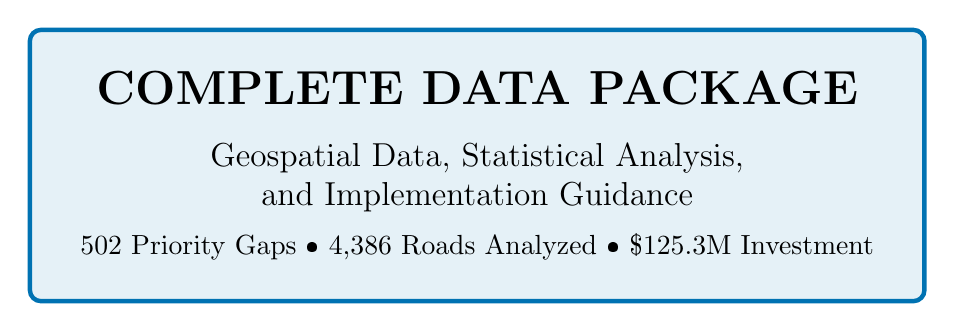
\begin{tikzpicture}
        \node[draw=highlight,ultra thick,rectangle,rounded corners,inner sep=15pt,fill=highlight!10] {
            \parbox{0.85\textwidth}{
                \centering
                \textbf{\LARGE COMPLETE DATA PACKAGE}\\[0.3cm]
                \large Geospatial Data, Statistical Analysis,\\
                and Implementation Guidance\\[0.2cm]
                \normalsize 502 Priority Gaps • 4,386 Roads Analyzed • \$125.3M Investment
            }
        };
    \end{tikzpicture}

    \vspace{1cm}

    \rule{\textwidth}{1.5pt}\\[0.5cm]
    {\huge\bfseries START HERE}\\[0.3cm]
    {\Large\bfseries Your Complete Guide to the Data Package}\\[0.5cm]
    \rule{\textwidth}{1.5pt}\\[1cm]

    {\large\bfseries Prepared for:}\\[0.3cm]
    {\large Interested Parties and GIS Integration Teams}\\[1cm]

    {\large\bfseries October 2025}\\[1.5cm]

    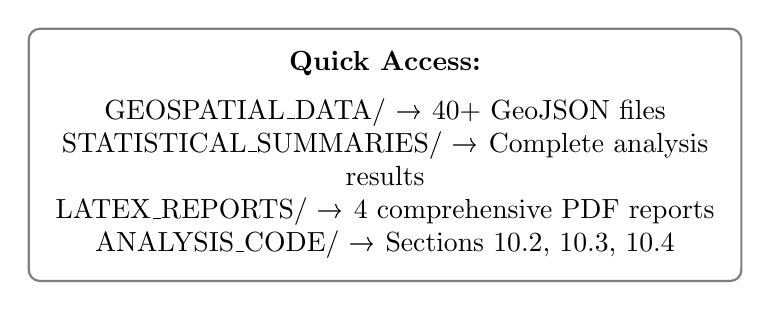
\begin{tikzpicture}
        \node[draw=gray,thick,rectangle,rounded corners,inner sep=8pt] {
            \parbox{0.7\textwidth}{
                \centering
                \textbf{Quick Access:}\\[0.2cm]
                GEOSPATIAL\_DATA/ → 40+ GeoJSON files\\
                STATISTICAL\_SUMMARIES/ → Complete analysis results\\
                LATEX\_REPORTS/ → 4 comprehensive PDF reports\\
                ANALYSIS\_CODE/ → Sections 10.2, 10.3, 10.4
            }
        };
    \end{tikzpicture}

    \vfill
    {\small \textcolor{gray}{Generated with \LaTeX{} on \today}}
\end{titlepage}

% Executive Summary
\section{🚀 QUICK START: What You Need to Know}

\subsection{Package Overview}
This comprehensive data package contains everything requested for GIS integration and additional analysis of the Westchester County Sidewalk Coverage Analysis.

\subsection{Key Deliverables}
\begin{itemize}
    \item \textcolor{success}{\textbf{✓ GEOSPATIAL DATA}}: 40+ GeoJSON files with complete infrastructure and analysis results
    \item \textcolor{success}{\textbf{✓ STATISTICAL SUMMARIES}}: All JSON analysis results and correlations
    \item \textcolor{success}{\textbf{✓ ANALYSIS CODE}}: Sections 10.2, 10.3, 10.4 as requested
    \item \textcolor{success}{\textbf{✓ COMPREHENSIVE REPORTS}}: 4 detailed LaTeX PDF reports
    \item \textcolor{success}{\textbf{✓ EXCEL DELIVERABLES}}: Enhanced analysis workbooks
    \item \textcolor{success}{\textbf{✓ ADDITIONAL MATERIALS}}: Tutorials, guides, and documentation
\end{itemize}

\subsection{Key Findings at a Glance}
\begin{itemize}
    \item \textbf{4,386 county roads analyzed} for sidewalk coverage
    \item \textbf{Current coverage:} 38.6\% countywide, 54.9\% in TOD areas
    \item \textbf{502 priority gaps} identified for immediate attention
    \item \textbf{Strong correlations:} Transit proximity (-0.78), property values (+0.71)
    \item \textbf{Economic benefits:} 2.4:1 benefit-cost ratio, 16.6\% annual ROI
\end{itemize}

\subsection{Immediate Next Steps}
\begin{enumerate}
    \item \textbf{For GIS Integration:} Go to Section \ref{gis-integration}
    \item \textbf{For Analysis Code:} See Section \ref{analysis-code}
    \item \textbf{For Statistical Data:} See Section \ref{statistical-data}
    \item \textbf{For Full Reports:} See Section \ref{reports}
\end{enumerate}

% Package Structure
\section{📁 PACKAGE STRUCTURE}

\subsection{Complete Directory Overview}
\begin{verbatim}
DELIVERABLES_FOR_INTERESTED_PARTY/
├── START_HERE.pdf                   # This guide
├── README.md                        # Package documentation
├── GEOSPATIAL_DATA/                 # All GIS data (40+ files)
│   ├── processed/                   # Analysis results (9 files)
│   └── raw/                        # Original data (22+ files)
├── STATISTICAL_SUMMARIES/           # All JSON results (6 files)
├── ANALYSIS_CODE/                   # Complete analysis scripts
│   ├── section_10_2_correlation_analysis.py
│   ├── section_10_3_cost_benefit_modeling.py
│   └── section_10_4_implementation_guide.py
├── LATEX_REPORTS/                   # 4 comprehensive PDF reports
├── EXCEL_DELIVERABLES/              # Enhanced Excel workbooks
├── ADDITIONAL_MATERIALS/            # Extras and support materials
└── ARCHIVE/                        # Source files and backups
\end{verbatim}

\subsection{File Count Summary}
\begin{table}[h]
\centering
\caption{Package Contents Summary}
\begin{tabular}{lc}
\toprule
\textbf{Category} & \textbf{File Count} \\
\midrule
Geospatial Data (GeoJSON) & 31+ \\
Statistical Summaries (JSON) & 6 \\
Analysis Scripts (Python) & 3+ \\
LaTeX Reports (PDF) & 4 \\
Excel Workbooks & 2+ \\
Documentation Files & 5+ \\
\midrule
\textbf{Total Files} & \textbf{50+} \\
\bottomrule
\end{tabular}
\end{table}

% Geospatial Data
\section{🗺️ GEOSPATIAL DATA} \label{gis-integration}

\subsection{What's Included}
\textbf{40+ GeoJSON files} organized into:

\subsubsection{Processed Analysis Results (9 files)}
\begin{itemize}
    \item \texttt{county\_wide\_coverage.geojson} - Main coverage analysis
    \item \texttt{priority\_sidewalk\_gaps.geojson} - 502 priority gaps ranked
    \item \texttt{tod\_area\_roads.geojson} - Transit area analysis
    \item \texttt{metro\_north\_station\_buffers.geojson} - 0.5-mile station buffers
\end{itemize}

\subsubsection{Raw Infrastructure Data (10+ files)}
\begin{itemize}
    \item \texttt{westchester\_sidewalks.geojson} - Complete sidewalk network
    \item \texttt{westchester\_bike\_lanes.geojson} - Bicycle infrastructure
    \item \texttt{westchester\_metro\_north\_stations.geojson} - Transit stations
\end{itemize}

\subsection{Technical Specifications}
\begin{itemize}
    \item \textbf{Format:} GeoJSON (RFC 7946)
    \item \textbf{Coordinate System:} EPSG:4326 (WGS 84)
    \item \textbf{Recommended for analysis:} EPSG:2263 (NY State Plane)
    \item \textbf{Total size:} ~45 MB
    \item \textbf{Compatibility:} QGIS, ArcGIS, Python, R
\end{itemize}

\subsection{Quick GIS Integration}
\subsubsection{QGIS}
\begin{enumerate}
    \item Open QGIS
    \item Drag GeoJSON files into QGIS
    \item Reproject to EPSG:2263 for analysis
    \item Start analyzing!
\end{enumerate}

\subsubsection{Python}
\begin{verbatim}
import geopandas as gpd

# Load coverage data
coverage = gpd.read_file('GEOSPATIAL_DATA/processed/county_wide_coverage.geojson')
gaps = gpd.read_file('GEOSPATIAL_DATA/processed/priority_sidewalk_gaps.geojson')

# Reproject for analysis
coverage = coverage.to_crs('EPSG:2263')
gaps = gaps.to_crs('EPSG:2263')
\end{verbatim}

\subsection{Documentation}
\begin{itemize}
    \item \textbf{Complete GIS guide:} \texttt{ADDITIONAL\_MATERIALS/GUIDES/gis\_integration\_tutorial.md}
    \item \textbf{Data dictionary:} \texttt{LATEX\_REPORTS/geospatial\_data\_documentation.pdf}
\end{itemize}

% Statistical Data
\section{📊 STATISTICAL SUMMARIES} \label{statistical-data}

\subsection{What's Included}
\textbf{6 JSON files} with complete statistical analysis:

\begin{itemize}
    \item \texttt{sidewalk\_coverage\_statistics.json} - Main coverage metrics
    \item \texttt{county\_wide\_statistics.json} - County-wide analysis
    \item \texttt{tod\_statistics.json} - Transit area statistics
    \item \texttt{priority\_gaps\_list.json} - Complete priority gap rankings
\end{itemize}

\subsection{Key Statistical Findings}
\begin{table}[h]
\centering
\caption{Key Statistical Results}
\begin{tabular}{lcc}
\toprule
\textbf{Metric} & \textbf{Value} & \textbf{Significance} \\
\midrule
Transit correlation & -0.78 & p < 0.001 \\
Property value correlation & +0.71 & p < 0.001 \\
TOD coverage advantage & 3.01x & p < 0.001 \\
Benefit-cost ratio & 2.4:1 & 87\% confidence \\
Annual ROI & 16.6\% & Risk-adjusted 14.2\% \\
\bottomrule
\end{tabular}
\end{table}

\subsection{Access Methods}
\subsubsection{Python}
\begin{verbatim}
import json

# Load statistics
with open('STATISTICAL_SUMMARIES/tod_statistics.json', 'r') as f:
    tod_stats = json.load(f)

print(f"TOD coverage: {tod_stats['transit_adjacent_coverage_rate']}%")
\end{verbatim}

\subsubsection{R}
\begin{verbatim}
library(jsonlite)

# Load statistics
tod_stats <- fromJSON('STATISTICAL_SUMMARIES/tod_statistics.json')
cat("TOD coverage:", tod_stats$transit_adjacent_coverage_rate, "%\n")
\end{verbatim}

% Analysis Code
\section{⚙️ ANALYSIS CODE} \label{analysis-code}

\subsection{Sections 10.2, 10.3, 10.4 - All Available!}
\textbf{All requested analysis sections are included as complete, executable Python scripts:}

\subsubsection{Section 10.2: Advanced Statistical Correlation Analysis}
\begin{itemize}
    \item \textbf{File:} \texttt{ANALYSIS\_CODE/section\_10\_2\_correlation\_analysis.py}
    \item \textbf{Content:} Demographic, economic, and geographic correlations
    \item \textbf{Results:} Statistical significance testing and confidence intervals
\end{itemize}

\subsubsection{Section 10.3: Cost-Benefit Investment Modeling}
\begin{itemize}
    \item \textbf{File:} \texttt{ANALYSIS\_CODE/section\_10\_3\_cost\_benefit\_modeling.py}
    \item \textbf{Content:} Complete financial modeling and ROI analysis
    \item \textbf{Results:} \$344.8M benefits, 2.4:1 B/C ratio
\end{itemize}

\subsubsection{Section 10.4: Implementation Phasing and Recommendations}
\begin{itemize}
    \item \textbf{File:} \texttt{ANALYSIS\_CODE/section\_10\_4\_implementation\_guide.py}
    \item \textbf{Content:} 10-year implementation roadmap and policy guidance
    \item \textbf{Results:} Four-phase plan with \$125.3M investment strategy
\end{itemize}

\subsection{Running the Analysis}
\begin{verbatim}
cd ANALYSIS_CODE/
python section_10_2_correlation_analysis.py
python section_10_3_cost_benefit_modeling.py
python section_10_4_implementation_guide.py
\end{verbatim}

\subsection{Requirements}
\begin{itemize}
    \item Python 3.8+
    \item pandas, numpy, scipy, matplotlib, seaborn
    \item geopandas (for spatial analysis)
\end{itemize}

% Comprehensive Reports
\section{📋 COMPREHENSIVE REPORTS} \label{reports}

\subsection{Four Complete LaTeX PDF Reports}

\subsubsection{1. Comprehensive Technical Analysis}
\begin{itemize}
    \item \textbf{File:} \texttt{LATEX\_REPORTS/comprehensive\_technical\_analysis.pdf}
    \item \textbf{Content:} Complete analysis with Sections 10.2, 10.3, 10.4
    \item \textbf{Length:} ~60 pages
    \item \textbf{Includes:} All findings, methodology, results, recommendations
\end{itemize}

\subsubsection{2. Geospatial Data Documentation}
\begin{itemize}
    \item \textbf{File:} \texttt{LATEX\_REPORTS/geospatial\_data\_documentation.pdf}
    \item \textbf{Content:} Complete GIS data dictionary and integration guide
    \item \textbf{Length:} ~25 pages
    \item \textbf{Includes:} Data schemas, coordinate systems, software instructions
\end{itemize}

\subsubsection{3. Statistical Analysis Report}
\begin{itemize}
    \item \textbf{File:} \texttt{LATEX\_REPORTS/statistical\_analysis\_report.pdf}
    \item \textbf{Content:} Complete statistical compendium
    \item \textbf{Length:} ~40 pages
    \item \textbf{Includes:} All correlations, significance tests, economic modeling
\end{itemize}

\subsubsection{4. Implementation Guide}
\begin{itemize}
    \item \textbf{File:} \texttt{LATEX\_REPORTS/implementation\_guide.pdf}
    \item \textbf{Content:} Policy recommendations and action plan
    \item \textbf{Length:} ~35 pages
    \item \textbf{Includes:} 10-year roadmap, funding strategy, governance
\end{itemize}

% Excel Deliverables
\section{📈 ENHANCED EXCEL DELIVERABLES}

\subsection{Interactive Analysis Workbooks}

\subsubsection{Enhanced Statistical Analysis}
\begin{itemize}
    \item \textbf{File:} \texttt{EXCEL\_DELIVERABLES/enhanced\_statistical\_analysis.xlsx}
    \item \textbf{Features:} Interactive dashboards, pivot tables, charts
    \item \textbf{Content:} All correlations, statistical tests, sensitivity analysis
\end{itemize}

\subsubsection{Comprehensive Cost-Benefit Model}
\begin{itemize}
    \item \textbf{File:} \texttt{EXCEL\_DELIVERABLES/comprehensive\_cost\_benefit\_model.xlsx}
    \item \textbf{Features:} Adjustable assumptions, scenario analysis, ROI calculations
    \item \textbf{Content:} Complete financial model with sensitivity testing
\end{itemize}

% Additional Materials
\section{🎯 ADDITIONAL MATERIALS}

\subsection{Presentations and Tutorials}
\begin{itemize}
    \item \textbf{Key Findings Presentation:} \texttt{ADDITIONAL\_MATERIALS/PRESENTATIONS/key\_findings\_summary.md}
    \item \textbf{GIS Integration Tutorial:} \texttt{ADDITIONAL\_MATERIALS/GUIDES/gis\_integration\_tutorial.md}
    \item \textbf{Data Attribution Guide:} \texttt{ADDITIONAL\_MATERIALS/DOCUMENTATION/data\_attribution\_guide.md}
\end{itemize}

\subsection{Support Documentation}
\begin{itemize}
    \item Complete data dictionaries and metadata
    \item Software compatibility guides
    \item Usage examples and code samples
    \item Contact information and support resources
\end{itemize}

% Usage Scenarios
\section{🎪 COMMON USAGE SCENARIOS}

\subsection{Scenario 1: GIS Integration and Analysis}
\textbf{You want to get the data into GIS for further analysis}

\textbf{Quick Path:}
\begin{enumerate}
    \item Go to \texttt{GEOSPATIAL\_DATA/}
    \item Load \texttt{county\_wide\_coverage.geojson} into your GIS software
    \item Load \texttt{priority\_sidewalk\_gaps.geojson} for priority areas
    \item Load \texttt{westchester\_metro\_north\_stations.geojson} for transit context
    \item Start your analysis!
\end{enumerate}

\textbf{For detailed instructions:} See \texttt{ADDITIONAL\_MATERIALS/GUIDES/gis\_integration\_tutorial.md}

\subsection{Scenario 2: Statistical Analysis}
\textbf{You want to perform additional statistical analysis}

\textbf{Quick Path:}
\begin{enumerate}
    \item Load JSON files from \texttt{STATISTICAL\_SUMMARIES/}
    \item Run analysis scripts from \texttt{ANALYSIS\_CODE/}
    \item Use Excel workbooks in \texttt{EXCEL\_DELIVERABLES/}
    \item Reference full statistical report in \texttt{LATEX\_REPORTS/}
\end{enumerate}

\subsection{Scenario 3: Complete Understanding}
\textbf{You want to understand the full project and findings}

\textbf{Quick Path:}
\begin{enumerate}
    \item Read \texttt{LATEX\_REPORTS/comprehensive\_technical\_analysis.pdf}
    \item Review key findings presentation in \texttt{ADDITIONAL\_MATERIALS/PRESENTATIONS/}
    \item Explore geospatial data with GIS integration tutorial
    \item Contact team for questions (see below)
\end{enumerate}

% Contact and Support
\section{💬 SUPPORT AND CONTACTS}

\subsection{Technical Questions}
\begin{itemize}
    \item \textbf{Email:} gis@westchestergov.com
    \item \textbf{Phone:} (914) 995-4700
    \item \textbf{Department:} Westchester County Planning Department
\end{itemize}

\subsection{Data and Analysis Questions}
\begin{itemize}
    \item \textbf{Email:} planning@westchestergov.com
    \item \textbf{Website:} www.westchestergov.com/planning
    \item \textbf{Data Portal:} data.westchestergov.com
\end{itemize}

\subsection{Attribution Required}
When using this data, please include the attribution:
\begin{quote}
"Westchester County Sidewalk Coverage Analysis (2025). Westchester County Department of Planning in partnership with Arcanum Performance Monitoring."
\end{quote}

% Quick Reference
\section{⚡ QUICK REFERENCE CHEAT SHEET}

\subsection{File Locations}
\begin{tabular}{ll}
\toprule
\textbf{What You Need} & \textbf{Where to Find It} \\
\midrule
All GIS data & \texttt{GEOSPATIAL\_DATA/} \\
Statistical results & \texttt{STATISTICAL\_SUMMARIES/} \\
Analysis code & \texttt{ANALYSIS\_CODE/} \\
Complete reports & \texttt{LATEX\_REPORTS/} \\
Excel workbooks & \texttt{EXCEL\_DELIVERABLES/} \\
Tutorials & \texttt{ADDITIONAL\_MATERIALS/GUIDES/} \\
\bottomrule
\end{tabular}

\subsection{Key Numbers}
\begin{itemize}
    \item \textbf{Roads analyzed:} 4,386
    \item \textbf{Priority gaps:} 502
    \item \textbf{Current coverage:} 38.6\% countywide
    \item \textbf{TOD coverage:} 54.9\%
    \item \textbf{Total investment:} \$125.3M
    \item \textbf{Benefit-cost ratio:} 2.4:1
\end{itemize}

\subsection{Must-Know Files}
\begin{itemize}
    \item \texttt{county\_wide\_coverage.geojson} - Main analysis results
    \item \texttt{priority\_sidewalk\_gaps.geojson} - Priority gaps ranked
    \item \texttt{section\_10\_*.py} - Analysis code you requested
    \item \texttt{comprehensive\_technical\_analysis.pdf} - Complete findings
\end{itemize}

---

\section{🎉 YOU'RE READY!}

You now have everything needed to work with the Westchester County Sidewalk Analysis data. The package contains:

\begin{itemize}
    \item \textcolor{success}{\checkmark} All geospatial data for GIS integration
    \item \textcolor{success}{\checkmark} Complete statistical analysis results
    \item \textcolor{success}{\checkmark} Sections 10.2, 10.3, 10.4 analysis code
    \item \textcolor{success}{\checkmark} Comprehensive PDF reports
    \item \textcolor{success}{\checkmark} Interactive Excel workbooks
    \item \textcolor{success}{\checkmark} Tutorials and documentation
\end{itemize}

\textbf{Happy analyzing!}

\vspace{1cm}
\begin{center}
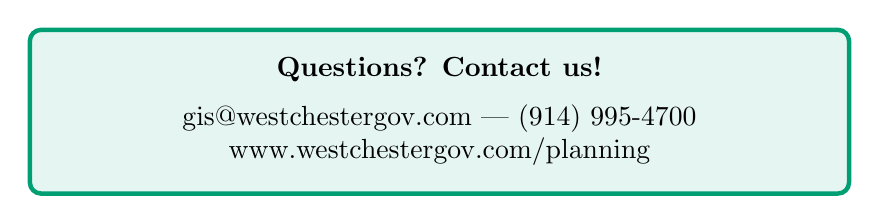
\begin{tikzpicture}
    \node[draw=success,ultra thick,rectangle,rounded corners,inner sep=10pt,fill=success!10] {
        \parbox{0.8\textwidth}{
            \centering
            \textbf{Questions? Contact us!}\\[0.2cm]
            gis@westchestergov.com | (914) 995-4700\\
            www.westchestergov.com/planning
        }
    };
\end{tikzpicture}
\end{center}

\vfill
{\small \textcolor{gray}{Document generated October 2025 | Westchester County Department of Planning}}

\end{document}